% !TeX program = lualatex
% !BIB program = biber
% Lualatex is important to render TTF fonts; with pdflatex it's just the regular one
% ratio 16:9 -- https://tex.stackexchange.com/questions/14336/

% compile two versions, inspired by https://tex.stackexchange.com/a/1501
% use the script "compile-pdf.sh"
\newif\ifhandout
% if flags.tex does not exist, create an empty file to be able to compile in TeXstudio
\input{flags}

\ifhandout
\documentclass[12pt,aspectratio=169,handout]{beamer}
\else
\documentclass[12pt,aspectratio=169]{beamer}
\fi



% TODO change "leftfootertext" to your liking
\newcommand{\leftfootertext}{\insertsubtitle}  % just the \title{} text by default
%\newcommand{\leftfootertext}{RNNs and encoder-decoder architectures}  % Your name, for instance


% ------- RUB specifics ----------
% adjust for 16:9
% https://tex.stackexchange.com/questions/354022/modifying-the-margins-of-all-slides-in-beamer
\setbeamersize{text margin left=0.3cm,text margin right=4.5cm} 


% use Metropolis as the basis theme
\usetheme[subsectionpage=progressbar]{metropolis}
% blocks with background globally
\metroset{block=fill}


\usepackage{fontspec}
% RUB fonts need to be installed
% 'UprightFont = * Light' makes sure that the base font is RubFlama Light, which looks
% lighter than RubFlama Regular (would be too thick for slides)
\setsansfont[Scale=MatchLowercase, UprightFont = * Light, BoldFont = * Bold]{RubFlama}
%\setsansfont{Arial} % Open source alternative if you don't have RubFlama

% RUB color scheme
% Dark blue: 0; 53; 96; #003560
\definecolor{RUBDarkBlue}{RGB}{0, 53, 96}

% Light yellow (table fill, etc.); 238; 250; 196; #EEFAC4
\definecolor{RUBLightYellow}{RGB}{238, 250, 196}

%Light green: 141; 174; 16
\definecolor{RUBLightGreen}{RGB}{141, 174, 16}


\setbeamercolor{titlelike}{fg=RUBDarkBlue}
\setbeamercolor{subtitle}{fg=RUBLightGreen}
\setbeamercolor{separation line}{fg=RUBLightGreen}
\setbeamercolor{frametitle}{bg=white, fg=RUBDarkBlue}

% horizontal line on title page and sections
\setbeamercolor{alerted text}{fg=RUBLightGreen}


% Adjust footer bottom (too large by default)
\setbeamertemplate{footline}{%
  \begin{beamercolorbox}[wd=\textwidth, sep=2ex]{footline}%
    \usebeamerfont{page number in head/foot}%
    \usebeamertemplate*{frame footer}
    \hfill%
    \usebeamertemplate*{frame numbering}
  \end{beamercolorbox}%
}


% Lab name, numbering, etc. in footer
\setbeamertemplate{frame numbering}{TrustHLT --- Prof.\ Dr.\ Ivan Habernal \hspace*{1ex} 
\includegraphics[width=7em]{img/rub-logo.pdf}\hspace*{1ex}}

\setbeamertemplate{frame footer}{\hspace*{1ex}\insertframenumber \hspace*{2ex} \leftfootertext}

% adjust the background to be completely white
\setbeamercolor{background canvas}{bg=white}

% logos on the title page
\titlegraphic{%
	\begin{picture}(0,0)
		\put(435,0){\makebox(0,0)[rt]{
\includegraphics[width=7em]{img/rub-logo.pdf}}}
		\put(435,-170){\makebox(0,0)[rt]{
\includegraphics[width=4em]{img/logo-trusthlt.pdf}}}
		\put(435,-196){\makebox(0,0)[rt]{
\includegraphics[width=9em]{img/logo-rctrust.pdf}}}
	\end{picture}%
}


% show TOC at every section start
\AtBeginSection{
	\frame{
		\vspace{2em}
		\sectionpage
		\hspace*{2.2em}\begin{minipage}{10cm}
			\tableofcontents[currentsection]
		\end{minipage}
	}
}

% TOC without subsection
\setcounter{tocdepth}{1} % only-- part,chapters,sections 

% bullet points: rectangles
\useinnertheme{rectangles}
\setbeamercolor{itemize item}{fg=RUBLightGreen}
\setbeamercolor{itemize subitem}{fg=RUBLightGreen}
% enumerate: blue background for better readability
\setbeamercolor{item projected}{bg=RUBDarkBlue}

% make boxes (example, block, etc.) background lighter for readability
\setbeamercolor{block title}{%
	use=normal text,
	fg=normal text.fg,
	bg=normal text.bg!90!fg % lighter background in block title
}
\setbeamercolor{block body}{
	use={block title, normal text},
	bg=block title.bg!30!normal text.bg % lighter background in block body
}


% RUB colors in blocks
\setbeamercolor{block title alerted}{%
	use={block title, alerted text},
	bg=RUBDarkBlue,
	%fg=RUBLightYellow % looks bad
	fg=white % better contrast
}

\setbeamercolor{block title example}{%
	use={block title, example text},
	fg=RUBLightGreen
}


% ------- end of RUB specifics ----------

% all itemize with pause by default
%\beamerdefaultoverlayspecification{<+->}


% typeset mathematics on serif
\usefonttheme[onlymath]{serif}

% better bibliography using biber as backend
\usepackage[natbib=true,backend=biber,style=authoryear-icomp,maxbibnames=30,maxcitenames=9,uniquelist=false,giveninits=true,doi=false,url=false,dashed=false,isbn=false]{biblatex}
% shared bibliography
\addbibresource{../bibliography.bib}
% disable "ibid" for repeated citations
\boolfalse{citetracker}



\usepackage{xspace}


% for derivatives, https://tex.stackexchange.com/a/412442
\usepackage{physics}

\usepackage{tikz}
\usetikzlibrary{matrix, positioning}
\usetikzlibrary{angles,quotes} % for angles
\usetikzlibrary{backgrounds} % background
\usetikzlibrary{decorations.pathreplacing} % curly braces
\usetikzlibrary{calligraphy}
\usetikzlibrary{calc} % for neural nets

% for plotting functions
\usepackage{pgfplots}
\usepgfplotslibrary{dateplot}

% sub-figures
\usepackage{caption}
\usepackage{subcaption}

% book tabs
\usepackage{booktabs}


% argmin, argmax
\usepackage{amsmath}
\DeclareMathOperator*{\argmax}{arg\!\max}
\DeclareMathOperator*{\argmin}{arg\!\min}
% softmax
\DeclareMathOperator*{\softmax}{soft\!\max}
% Mask
\DeclareMathOperator*{\mask}{mask}

% bold math
\usepackage{bm}

% for \mathclap
\usepackage{mathtools}

% algorithms
\usepackage[noend]{algpseudocode}


% for neurons and layers in tikz
\tikzset{
	neuron/.style={draw, rectangle, inner sep=2pt, minimum width=0.75cm, fill=blue!20},
	param/.style={draw, rectangle, inner sep=2pt, minimum width=0.75cm, fill=green!20},
	constant/.style={draw, rectangle, inner sep=2pt, minimum width=0.75cm, fill=black!15},
	% for citation nodes right top
	ref/.style={anchor = north east, text width=7.8cm, yshift=-1.3cm, xshift=-0.2cm, scale=0.5},
	state/.style={rectangle, inner sep=2pt, minimum width=0.75cm, fill=black!5},
}

% added in lecture 10
\tikzset{
	mtx/.style={
		matrix of math nodes,
		left delimiter={[}, right delimiter={]}
	},
	hlt/.style={opacity=0.1, line width=4 mm, line cap=round},
	hltr/.style={opacity=0.5, rounded corners=2pt, inner sep=-1pt}
}

% for strike-through text (added in Lecture 06)
\usepackage[normalem]{ulem}

% added in Lecture 7
% RNN
\DeclareMathOperator*{\rnn}{RNN}
% RNN star
\DeclareMathOperator*{\rnnstar}{RNN^{*}}
% bi-RNN
\DeclareMathOperator*{\birnn}{biRNN}


% added in Lecture 9
\usetikzlibrary{fit} % for hightligting by calling "fit"

% algorithms
\usepackage[noend]{algpseudocode}



\title{Privacy-Preserving Natural Language Processing}
\subtitle{Lecture 3 -- Introduction to Differential Privacy}
\date{April 24, 2025}
\author{Prof.\ Dr.\ Ivan Habernal}
\institute{
\texttt{www.trusthlt.org} \\
Chair of Trustworthy Human Language Technologies (TrustHLT) \\
Ruhr University Bochum \& Research Center Trustworthy Data Science and Security}

\begin{document}

\maketitle


\section{Intro}

\begin{frame}{Overview}

Last lecture: Towards probabilistic approach to privacy

This lecture: Formalizing differential privacy, introducing some basic algorithms

%\begin{tikzpicture}[overlay, remember picture]
%\node at (current page.north east)[ref] {
%\fullcite{Voigt.Bussche.2017} \par};
%\end{tikzpicture}
\end{frame}


\section{Recap Lecture 3}

\begin{frame}{Example: How many persons in the database take illegal drugs?}

\begin{table}
\footnotesize
\begin{tabular}{lrrr} \toprule
Name & Hospitalized in year & Age & Illegal drug use \\ \midrule
Alice & 2024 & 32 & yes \\
Bob & 2020 & 21 & no \\
Charlie & 2023 & 45 & no \\
$\ldots$ & & & \\
Xander & 2020 & 31 & yes \\ \bottomrule
\end{tabular}
\end{table}

What might be public information: the size of the dataset (say $n = 100$)

The true answer to the query: 2

If Xander reveals his drug use, and we know Alice is in the database, her privacy is revealed!

%\begin{tikzpicture}[overlay, remember picture]
%\node at (current page.north east)[ref] {
%\fullcite{Voigt.Bussche.2017} \par};
%\end{tikzpicture}\
\end{frame}


\begin{frame}{Irreversibly alter the true query result by randomness}

The randomized output should be likely close to the true value, and unlikely far away

We picked the Laplace distribution with scale $b = 1$

We explored two possible scenarios
\begin{itemize}
	\item $D$: Alice was in the dataset (and then querying)
	\item $D'$: Alice was removed from the dataset (and then querying)
\end{itemize}

\end{frame}


\begin{frame}{For any observed $y$, was it sampled from $Y$ or from $Y'$?}

The underlying database was $D$ for $Y$ and $D'$ for $Y'$, respectively

$$
\frac{\Pr[Y = y]}{\Pr[Y' = y]} \leq \exp(1) \qquad
\frac{\Pr[Y' = y]}{\Pr[Y = y]} \leq \exp(1)
$$

No matter what value we get after privatizing the counting query -- we can only get some limited "information" about whether it came from $Y$ or $Y'$.

\end{frame}



\begin{frame}{Summary}

Four counting queries, the maximum difference of the query result is 1 (when a particular person is not in the dataset)

Scale $b = 1$ for the Laplace distribution gives us the following upper bound on privacy loss

$
\frac{\Pr[Y = y]}{\Pr[Y' = y]} \leq \exp(1) \qquad
\frac{\Pr[Y' = y]}{\Pr[Y = y]} \leq \exp(1)
$

\end{frame}


\section{Neighboring datasets}

\begin{frame}{Defining neighboring datasets}
	
We saw that the bound was `symmetric'
$$
\frac{\Pr[Y = y]}{\Pr[Y' = y]} \leq \exp(1) \qquad
\frac{\Pr[Y' = y]}{\Pr[Y = y]} \leq \exp(1)
$$
On the left: One entry less in the denominator (= one entry more in the nominator)

On the right: One entry less in the nominator (= one entry more in the denominator)

The bound holds for any two datasets that \textbf{differ in the presence of one entry} (e.g., one row removed, or on row added) $\rightarrow$ \textbf{neighboring datasets}


\end{frame}

\begin{frame}{Neighboring dataset examples (choice of Alice is arbitrary!)}


\begin{table}
	\footnotesize
	\begin{tabular}{lrrr} \toprule
		Name & Hospitalized in year & Age & Illegal drug use \\ \midrule
		Alice & 2024 & 32 & yes \\
		Bob & 2020 & 21 & no \\
		Charlie & 2023 & 45 & no \\ \bottomrule
	\end{tabular}
	\caption{Database 1, including Alice}
\end{table}

\begin{table}
	\footnotesize
	\begin{tabular}{lrrr} \toprule
		Name & Hospitalized in year & Age & Illegal drug use \\ \midrule
		Bob & 2020 & 21 & no \\
		Charlie & 2023 & 45 & no \\ \bottomrule
	\end{tabular}
	\caption{Database 2, excluding Alice}
\end{table}
	
\end{frame}

\begin{frame}{Neighboring dataset examples}

Databases 1 and 2 from the previous slide are \textbf{neighboring} as they differ in presence or absence of a single row

We might denote them 1: $D$ and 2: $D'$ but this is an \textbf{arbitrary choice}

The neighboring dataset definition allows us to simplify
$$
\frac{\Pr[Y = y]}{\Pr[Y' = y]} \leq \exp(1) \qquad
\frac{\Pr[Y' = y]}{\Pr[Y = y]} \leq \exp(1)
$$
into one inequality (where again $Y$ is a random variable based on $D$ and $Y'$ is a random variable based on $D'$)
$$
\frac{\Pr[Y = y]}{\Pr[Y' = y]} \leq \exp(1)
$$

\end{frame}

\begin{frame}{Restating our bound with neighboring datasets}

Neighboring datasets = presence or absence of a single individual

Our bound $\frac{\Pr[Y = y]}{\Pr[Y' = y]} \leq \exp(1)$ holds for any neighboring datasets (we proved it, but convince yourself again)

So the absence or presence of \textbf{any single individual}
\begin{itemize}
	\item will influence the result of the counting query (but we want to keep this influence small $\rightarrow$ \textbf{utility})
	\item for any `all-mighty' adversary, the likelihood to find out the extra person's `private bit' (e.g., drug use) is upper bounded (the person wants to keep this bound small $\rightarrow$ \textbf{privacy})
\end{itemize}

\end{frame}



\section{Controlling privacy strength}

\begin{frame}{What if $\exp(1)$ is not strong enough?}

For $y \sim y_{\mathrm{true}} + \textrm{Lap}(b=1)$

The likelihood for preferring one hypothesis over the other	
$$
\frac{\Pr[Y = y]}{\Pr[Y' = y]} \leq \exp(1) \approx 2.718
$$

What would be the minimum of $\frac{\Pr[Y = y]}{\Pr[Y' = y]}$?

What would be the maximum of $\frac{\Pr[Y = y]}{\Pr[Y' = y]}$?

\pause

$$1 \leq \frac{\Pr[Y = y]}{\Pr[Y' = y]} \leq \infty$$
Why?

	
\end{frame}




\begin{frame}{Playing with the scale parameter $b$}

For $y \sim y_{\mathrm{true}} + \textrm{Lap}(\mu = 0; b=1)$


\begin{figure}
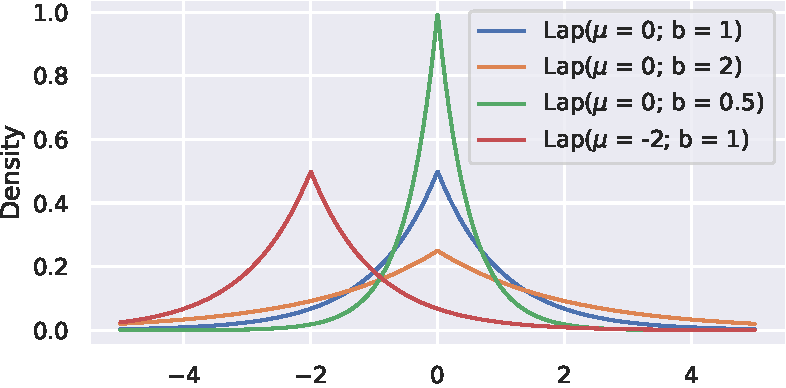
\includegraphics[width=0.6\linewidth]{img/laplace-distributions.pdf}
\caption{Laplace PDF (probability density function)}
\end{figure}
$
\textrm{Lap}(x; \mu, b) = \frac{1}{2b} \exp \left( - \frac{\abs{x - \mu}}{b}  \right)
$

What to do with the scale for stronger privacy?
	
\end{frame}


\begin{frame}{Intuition: Larger $b$ gives stronger privacy}

\begin{figure}
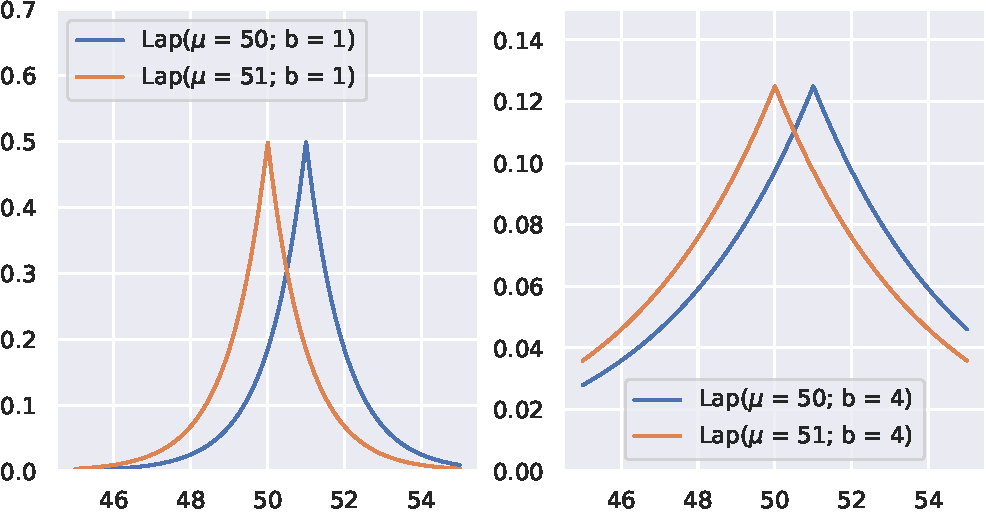
\includegraphics[width=0.9\linewidth]{img/laplace-grid1.pdf}
\caption{Laplace PDF (probability density function)}
\end{figure}
	
\end{frame}


\begin{frame}{How does that relate to the maximum privacy loss?}
Recall: likelihood of any output (x-axis) coming from $D'$ as opposed do $D$ (and vice versa)

\begin{figure}
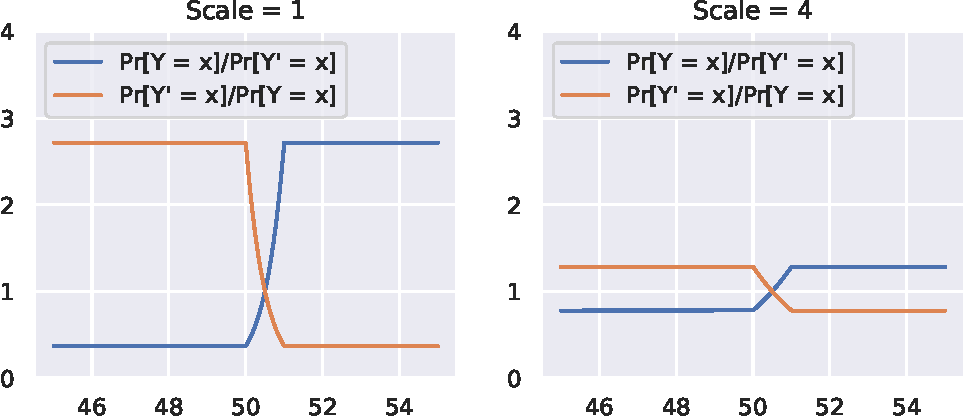
\includegraphics[width=0.9\linewidth]{img/privacy-loss1.pdf}
\caption{Privacy loss for two Laplace distributions for a counting query, varying scale $b$}
\end{figure}

\end{frame}



\begin{frame}{Let's try to formalize our intuition}

Counting query true value $y= 51$, one person removed $y = 50$
$$
\begin{aligned}
\frac{\Pr[Y = y]}{\Pr[Y' = y]} =
\frac{
\frac{1}{2b} \exp \left(- \frac{1}{b} \abs{y - 51} \right)
}{
\frac{1}{2b} \exp \left(- \frac{1}{b} \abs{y - 50} \right) 
}
&= \exp (\frac{1}{b} \abs{y - 50} - \abs{y - 51} ) \\
&\leq \exp (\frac{1}{b} \abs{(y - 50) - (y - 51)} ) \\
&= \exp (\frac{1}{b} \abs{y - 50 - y + 51} ) \\
&= \exp (\frac{1}{b} \abs{1}) = \exp(\frac{1}{b}) \\
\end{aligned}
$$
Will be the same for $\frac{\Pr[Y' = y]}{\Pr[Y = y]}$ (prove it!)

\end{frame}



\begin{frame}{Proof from the previous slide (added post-lectures 2024-07-15)}

$$
\begin{aligned}
\frac{\Pr[Y' = y]}{\Pr[Y = y]} =
\frac{
\frac{1}{2b} \exp \left(- \frac{1}{b} \abs{y - 50} \right)
}{
\frac{1}{2b} \exp \left(- \frac{1}{b} \abs{y - 51} \right)
}
&= \exp (\frac{1}{b} \abs{y - 51} - \abs{y - 50} ) \\
&\leq \exp (\frac{1}{b} \abs{(y - 51) - (y - 50)} ) \\
&= \exp (\frac{1}{b} \abs{y - 51 - y + 50} ) \\
&= \exp (\frac{1}{b} \abs{-1}) = \exp(\frac{1}{b}) \\
\end{aligned}
$$

\end{frame}




\begin{frame}{What have we discovered so far}

Our choice of 50 and 51 was arbitrary, the same proof will hold for any true answers differing by 1

For a \textbf{counting query}, the database curator (\textbf{trusted curator}, trusted holder) protects privacy of each individual by reporting
$$y \sim y_{\mathrm{true}} + \textrm{Lap}(b)$$

This ensures that for \textbf{any two neighboring datasets} the privacy loss is \textbf{bounded}

$$
\frac{\Pr[Y = y]}{\Pr[Y' = y]} \leq \exp(\frac{1}{b})
$$

\end{frame}




\section{Formalizing differential privacy}



\begin{frame}{Let's generalize our findings}

We had $\frac{\Pr[Y = y]}{\Pr[Y' = y]} \leq \exp(\frac{1}{b})$

We saw, that $\frac{1}{b}$ controls the strength of privacy. Let's generalize this notion and call it

\begin{block}{Privacy budget}
Denoted as $\varepsilon \in [0, \infty)$

$\varepsilon = 0$ is complete privacy but everything would be completely random

$\varepsilon = \infty$ is no privacy whatsoever
\end{block}
So for our counting query example, we would have
$\frac{\Pr[Y = y]}{\Pr[Y' = y]} \leq \exp(\varepsilon)$ where $\varepsilon = \frac{1}{b}$
\end{frame}


\begin{frame}{Let's formalize pure differential privacy}

Let's just rewrite $\frac{\Pr[Y = y]}{\Pr[Y' = y]} \leq \exp(\varepsilon)$:
$$
\Pr[Y = y] \leq \exp(\varepsilon) \Pr[Y' = y]
$$

Let's generalize the random variables $Y$ and $Y'$ by saying thery are \textbf{random variables parametrized by the dataset} (randomized algorithms, \textbf{randomized mechanisms}), e.g., $\mathcal{M}(D)$ or $\mathcal{M}(D')$
$$
\Pr[\mathcal{M}(D) = y] \leq \exp(\varepsilon) \Pr[\mathcal{M}(D') = y]
$$
\end{frame}


\begin{frame}{Let's formalize pure differential privacy}
We had $\Pr[\mathcal{M}(D) = y] \leq \exp(\varepsilon) \Pr[\mathcal{M}(D') = y]$

To make this defintion work for \textbf{any} random variable (categorical, discrete finite, countably infinite, uncounble), we must generalize the co-domain of $\mathcal{M}$

The co-domain of $\mathcal{M}(D)$ can be some arbitrary set $\mathcal{Z}$

We want that our privacy guarantees hold for \textbf{any possible output} $\mathcal{Y}$ which is any subset of the co-domain, i.e. $\mathcal{Y} \subseteq \mathcal{Z}$:
$$
\Pr[\mathcal{M}(D) \in \mathcal{Y}] \leq \exp(\varepsilon) \Pr[\mathcal{M}(D') \in \mathcal{Y}]
$$

\begin{tikzpicture}[overlay, remember picture]
\node at (current page.north east)[ref] {
\fullcite[Definition~2.4]{Dwork.Roth.2013} \par};
\end{tikzpicture}

\end{frame}


\begin{frame}{$(\varepsilon, 0)$ differential privacy (aka.\ pure DP)}

A randomized algorithm (mechanism) $\mathcal{M}$ is $(\varepsilon, 0)$-\textbf{differentially private} if for any two neighboring datasets $D, D'$ and any output $\mathcal{Y} \subseteq \mathcal{Z}$ this guarantee holds:
$$
\Pr[\mathcal{M}(D) \in \mathcal{Y}] \leq \exp(\varepsilon) \Pr[\mathcal{M}(D') \in \mathcal{Y}]
$$

\begin{tikzpicture}[overlay, remember picture]
\node at (current page.north east)[ref] {
\fullcite[Definition~2.4]{Dwork.Roth.2013} \par};
\end{tikzpicture}

\end{frame}


\section{Examples of $(\varepsilon, 0)$-DP mechanisms}


\begin{frame}{Laplace mechanism for counting query is $(\varepsilon, 0)$-DP}

Counting query: Report a number of persons with a certain attribute

Draw a random number $y_{\mathrm{lap}} \sim \textrm{Lap}(\mu = 0; b=\frac{1}{\varepsilon})$

Report $y = y_{\mathrm{true}} + y_{\mathrm{lap}}$


Proof: We did it already! (but practice it now backwards from the definition)

\begin{tikzpicture}[overlay, remember picture]
\node at (current page.north east)[ref] {
\fullcite[Definition~2.4]{Dwork.Roth.2013} \par};
\end{tikzpicture}

\end{frame}


\section{General numeric queries}

\begin{frame}{From counting query to numeric query}

Counting query: Report a number of persons with certain attribute(s)
$$
f: \mathcal{X} \mapsto \mathcal{Y} \subseteq \mathbb{N}
$$

Real-valued query: Report any value computed over certain attribute(s)
$$
f: \mathcal{X} \mapsto \mathcal{Y} \subseteq \mathbb{R}
$$

\end{frame}

\begin{frame}{Working example of numeric query}

\begin{table}
\footnotesize
\begin{tabular}{lr} \toprule
Name & Debt (in \texteuro) \\ \midrule
Alice & 2,800,798.00 \\
Bob & 7,000.00 \\
Charlie & 1.56 \\
Xander & 0.00 \\
\bottomrule
\end{tabular}
\caption{Debts of account holders in a bank}
\end{table}

Important constraint: Maximum debt the bank offers per person is 10,000,000 \texteuro


Query: What is the total debt in \texteuro?

\end{frame}



\begin{frame}{Naive attempt with the Laplace mechanism for counting queries}

\begin{block}{Laplace mechanism for counting query}
Draw $y_{\mathrm{lap}} \sim \textrm{Lap}(\mu = 0; b=\frac{1}{\varepsilon})$ and report $y = y_{\mathrm{true}} + y_{\mathrm{lap}}$
\end{block}

Will it ensure $\Pr[\mathcal{M}(D) \in \mathcal{Y}] \leq \exp(\varepsilon) \Pr[\mathcal{M}(D') \in \mathcal{Y}]$ for all neighboring datasets and any outputs?

\begin{table}
\footnotesize
\begin{tabular}{lr} \toprule
Name & Debt (in \texteuro) \\ \midrule
Alice & 2,800,798.00 \\
Bob & 7,000.00 \\
Charlie & 1.56 \\
Xander & 0.00 \\
\bottomrule
\end{tabular}
\end{table}

\end{frame}



\begin{frame}{Naive attempt with the Laplace mechanism for counting queries}

\begin{table}
\footnotesize
\begin{tabular}{lr} \toprule
Name & Debt (in \texteuro) \\ \midrule
Alice & 2,800,798.00 \\
Bob & 7,000.00 \\
Charlie & 1.56 \\
Xander & 0.00 \\
\bottomrule
\end{tabular}
\end{table}

Let's try for $D = \{A, B, C, X\}$ and $D' = \{B, C, X\}$

\begin{itemize}
\item $y_{\mathrm{true}}(D) = 2,807,799.56$
\item $y_{\mathrm{true}}(D') = 7,001.56$
\end{itemize}

\end{frame}



\begin{frame}{Naive solution with the Laplace mechanism for counting queries}

We had $y_{\mathrm{true}}(D) = 2,807,799.56$, $y_{\mathrm{true}}(D') = 7,001.56$

$$
\begin{aligned}
\frac{\Pr[Y = y]}{\Pr[Y' = y]} &=
\frac{
\frac{1}{2\frac{1}{\varepsilon}} \exp \left(- \frac{1}{\frac{1}{\varepsilon}} \abs{y - 2,807,799.56} \right)
}{
\frac{1}{2\frac{1}{\varepsilon}} \exp \left(- \frac{1}{\frac{1}{\varepsilon}} \abs{y - 7,001.56} \right) 
}
=
\frac{
\exp \left(- \varepsilon \abs{y - 2,807,799.56} \right)
}{
\exp \left(- \varepsilon \abs{y - 7,001.56} \right) 
} \\
&=
\exp \left\{ \varepsilon
\underbrace{
\left( \abs{y - 7,001.56} - \abs{y - 2,807,799.56} \right)
}_{\text{Exceeds 1 for some large } y}
\right\} \\
& \nleq \exp(\varepsilon) \\
\end{aligned}
$$
This naive solution violates DP! How to fix this?
\end{frame}


\section{Where we finished last time}


\begin{frame}{Recall: $(\varepsilon, 0)$ differential privacy (aka.\ pure DP)}

A randomized algorithm (mechanism) $\mathcal{M}$ is $(\varepsilon, 0)$-\textbf{differentially private} if for any two neighboring datasets $D, D'$ and any output $\mathcal{Y} \subseteq \mathcal{Z}$ this guarantee holds:
$$
\Pr[\mathcal{M}(D) \in \mathcal{Y}] \leq \exp(\varepsilon) \Pr[\mathcal{M}(D') \in \mathcal{Y}]
$$

\begin{tikzpicture}[overlay, remember picture]
\node at (current page.north east)[ref] {
\fullcite[Definition~2.4]{Dwork.Roth.2013} \par};
\end{tikzpicture}

\end{frame}


\begin{frame}{Recap: From counting query to numeric query}

Counting query: Report a number of persons with certain attribute(s)
$$
f: \mathcal{X} \mapsto \mathcal{Y} \subseteq \mathbb{N}
$$

Real-valued query: Report any value computed over certain attribute(s)
$$
f: \mathcal{X} \mapsto \mathcal{Y} \subseteq \mathbb{R}
$$

\end{frame}

\begin{frame}{Recap: Working example of numeric query}

\begin{table}
\footnotesize
\begin{tabular}{lr} \toprule
Name & Debt (in \texteuro) \\ \midrule
Alice & 2,800,798.00 \\
Bob & 7,000.00 \\
Charlie & 1.56 \\
Xander & 0.00 \\
\bottomrule
\end{tabular}
\caption{Debts of account holders in a bank}
\end{table}

Important constraint: Maximum debt the bank offers per person is 10,000,000 \texteuro


Query: What is the total debt in \texteuro?

\end{frame}



\begin{frame}{Recap: Naive attempt using the Laplace mechanism for counting queries}

\begin{block}{This approach failed}
Draw $y_{\mathrm{lap}} \sim \textrm{Lap}(\mu = 0; b=\frac{1}{\varepsilon})$ and report $y = y_{\mathrm{true}} + y_{\mathrm{lap}}$
\end{block}

Will it ensure $\Pr[\mathcal{M}(D) \in \mathcal{Y}] \leq \exp(\varepsilon) \Pr[\mathcal{M}(D') \in \mathcal{Y}]$ for all neighboring datasets and any outputs?

\begin{table}
\footnotesize
\begin{tabular}{lr} \toprule
Name & Debt (in \texteuro) \\ \midrule
Alice & 2,800,798.00 \\
Bob & 7,000.00 \\
Charlie & 1.56 \\
Xander & 0.00 \\
\bottomrule
\end{tabular}
\end{table}

\end{frame}



\begin{frame}{Recap: Naive attempt with the Laplace mechanism for counting queries}

\begin{table}
\footnotesize
\begin{tabular}{lr} \toprule
Name & Debt (in \texteuro) \\ \midrule
Alice & 2,800,798.00 \\
Bob & 7,000.00 \\
Charlie & 1.56 \\
Xander & 0.00 \\
\bottomrule
\end{tabular}
\end{table}

Let's try for $D = \{A, B, C, X\}$ and $D' = \{B, C, X\}$

\begin{itemize}
\item $y_{\mathrm{true}}(D) = 2,807,799.56$
\item $y_{\mathrm{true}}(D') = 7,001.56$
\end{itemize}

\end{frame}



\begin{frame}{Recap: Naive solution with the Laplace mechanism for counting queries}

We had $y_{\mathrm{true}}(D) = 2,807,799.56$, $y_{\mathrm{true}}(D') = 7,001.56$

$$
\begin{aligned}
\frac{\Pr[Y = y]}{\Pr[Y' = y]} &=
\frac{
\frac{1}{2\frac{1}{\varepsilon}} \exp \left(- \frac{1}{\frac{1}{\varepsilon}} \abs{y - 2,807,799.56} \right)
}{
\frac{1}{2\frac{1}{\varepsilon}} \exp \left(- \frac{1}{\frac{1}{\varepsilon}} \abs{y - 7,001.56} \right) 
}
=
\frac{
\exp \left(- \varepsilon \abs{y - 2,807,799.56} \right)
}{
\exp \left(- \varepsilon \abs{y - 7,001.56} \right) 
} \\
&=
\exp \left\{ \varepsilon
\underbrace{
\left( \abs{y - 7,001.56} - \abs{y - 2,807,799.56} \right)
}_{\text{Exceeds 1 for some large } y}
\right\} \\
& \nleq \exp(\varepsilon) \\
\end{aligned}
$$
This naive solution violates DP! How to fix this?
\end{frame}


%\section{Today}
%\begin{frame}{Outline}
%Fixing numeric query -- Introducing global L1 sensitivity
%The Laplace mechanism for numeric queries (including general proof)
%(?) Utility/error of Laplace mechanism?
%(?) Applications of Laplace mechanisms in NLP
%Exponential mechanism (including general proof)
%\end{frame}


\section{Global $\ell_1$ sensitivity}

\begin{frame}{How different neighboring datasets influence the output}
\begin{table}
\footnotesize
\begin{tabular}{lr} \toprule
Name & Debt (in \texteuro) \\ \midrule
Alice & 2,800,798.00 \\
Bob & 7,000.00 \\
Charlie & 1.56 \\
Xander & 0.00 \\
\bottomrule
\end{tabular}
\end{table}
$D = \{A, B, C, X\}$
\begin{itemize}
\item $D' = \{B, C, X\} = D \setminus \{A\}$
\begin{itemize}
\item $y_{\mathrm{true}}(D) = 2,807,799.56$
\item $y_{\mathrm{true}}(D') = 7,001.56$
\item $y_{\mathrm{true}}(D) - y_{\mathrm{true}}(D') = 2,800,798$
\end{itemize}
\end{itemize}
\end{frame}


\begin{frame}{How different neighboring datasets influence the output}
\begin{table}
\footnotesize
\begin{tabular}{lr} \toprule
Name & Debt (in \texteuro) \\ \midrule
Alice & 2,800,798.00 \\
Bob & 7,000.00 \\
Charlie & 1.56 \\
Xander & 0.00 \\
\bottomrule
\end{tabular}
\end{table}
\begin{itemize}
\item $D' = D \setminus \{B\}$
\begin{itemize}
\item $y_{\mathrm{true}}(D) = 2,807,799.56$
\item $y_{\mathrm{true}}(D') = 2,800,799.56$
\item $y_{\mathrm{true}}(D) - y_{\mathrm{true}}(D') = 7,000$
\end{itemize}
\end{itemize}
You should now see the pattern for this sum query
\end{frame}


\begin{frame}{How different neighboring datasets influence the output}
\begin{table}
\footnotesize
\begin{tabular}{lr} \toprule
Name & Debt (in \texteuro) \\ \midrule
Alice & 2,800,798.00 \\
Bob & 7,000.00 \\
Charlie & 1.56 \\
Xander & 0.00 \\
\bottomrule
\end{tabular}
\end{table}
\begin{itemize}
\item $D' = D \setminus \{A\}$:  $y_{\mathrm{true}}(D) - y_{\mathrm{true}}(D') = 2,800,798$
\item $D' = D \setminus \{B\}$: $y_{\mathrm{true}}(D) - y_{\mathrm{true}}(D') = 7,000$
\item $D' = D \setminus \{C\}$: $y_{\mathrm{true}}(D) - y_{\mathrm{true}}(D') = 1.56$
\item $D' = D \setminus \{X\}$: $y_{\mathrm{true}}(D) - y_{\mathrm{true}}(D') = 0$
\end{itemize}
Each person can change the result of the query by its value

Can we use this max value to fix our problem?

\end{frame}


\begin{frame}{Rescale the Laplace distribution}

\begin{block}{Previous attempt}
We had $y_{\mathrm{true}}(D) = 2,807,799.56$, $y_{\mathrm{true}}(D') = 7,001.56$
$$
\begin{aligned}
\frac{\Pr[Y = y]}{\Pr[Y' = y]} &=
\frac{
\frac{1}{2\frac{1}{\varepsilon}} \exp \left(- \frac{1}{\frac{1}{\varepsilon}} \abs{y - 2,807,799.56} \right)
}{
\frac{1}{2\frac{1}{\varepsilon}} \exp \left(- \frac{1}{\frac{1}{\varepsilon}} \abs{y - 7,001.56} \right) 
} \\
&=
\exp \left\{ \varepsilon
\underbrace{
\left( \abs{y - 7,001.56} - \abs{y - 2,807,799.56} \right)
}_{\text{Exceeds 1 for some large } y}
\right\} \\
& \nleq \exp(\varepsilon) \\
\end{aligned}
$$
\end{block}
How to make the term $\leq 1$?
\end{frame}


\begin{frame}{Rescale the Laplace distribution}

How to make the term $\leq 1$?
$$
\abs{y - 7,001.56} - \abs{y - 2,807,799.56}
$$

\begin{block}{Recall: Triangle inequality}
$a, b \in \mathbb{R}$:
$\abs{a} - \abs{b} \leq \abs{a- b}$
\end{block}
$$
\begin{aligned}
\abs{y - 7,001.56} - \abs{y - 2,807,799.56} &\leq \abs{(y - 7,001.56) - (y - 2,807,799.56)} \\
%\abs{y - 7,001.56} - \abs{y - 2,807,799.56} &\leq \abs{-7,001.56 + 2,807,799.56} \\
\abs{y - 7,001.56} - \abs{y - 2,807,799.56} &\leq 2,800,798 \text{ (Alice's value!)} \\
\frac{
\abs{y - 7,001.56} - \abs{y - 2,807,799.56}
}{2,800,798} &\leq 1 \\
\end{aligned}
$$
Now plug it back

\end{frame}



\begin{frame}{Rescale the Laplace distribution}


$$
\begin{aligned}
\frac{\Pr[Y = y]}{\Pr[Y' = y]} &=
\frac{
\frac{1}{2\frac{1}{\varepsilon}} \exp \left(- \frac{1}{\frac{1}{\varepsilon}}
\frac{
\abs{y - 2,807,799.56}
}{2,800,798}
\right)
}{
\frac{1}{2\frac{1}{\varepsilon}} \exp \left(- \frac{1}{\frac{1}{\varepsilon}}
\frac{
\abs{y - 7,001.56}
}{2,800,798}
\right) 
} \\
&=
\exp \left\{ \varepsilon
\frac{
\left( \abs{y - 7,001.56} - \abs{y - 2,807,799.56} \right)
}{2,800,798}
\right\} \\
& \leq \exp(\varepsilon) \\
\end{aligned}
$$

By scaling the Laplace distribution proportionally to the difference we achieved privacy (for this particular $D$ and $D'$ only!)
\end{frame}


\begin{frame}{Will it work for the worst case scenario?}

Remember: we said the maximum debt the bank offers per person is 10,000,000 \texteuro

We need to protect privacy even in the worst case, even when one person is a complete outlier

\begin{table}
\begin{tabular}{lr} \toprule
Name & Debt (in \texteuro) \\ \midrule
Alice & 0 \\
Bob & 0 \\
Charlie & 0 \\
Xander & 10,000,000 \\
\bottomrule
\end{tabular}
\end{table}


\end{frame}


\begin{frame}{Our previous scale $2,800,798$ would not be enough}

Let $D = \{A, B, C, X\}$, $D' = \{A, B, C\}$

$y_{\mathrm{true}}(D) = 10,000,000$, $y_{\mathrm{true}}(D') = 0$


$$
\begin{aligned}
\frac{\Pr[Y = y]}{\Pr[Y' = y]} &=
\frac{
\frac{1}{2\frac{1}{\varepsilon}} \exp \left(- \frac{1}{\frac{1}{\varepsilon}}
\frac{
\abs{y - 10,000,000}
}{2,800,798}
\right)
}{
\frac{1}{2\frac{1}{\varepsilon}} \exp \left(- \frac{1}{\frac{1}{\varepsilon}}
\frac{
\abs{y - 0}
}{2,800,798}
\right) 
} \\
&=
\exp \left\{ \varepsilon
\underbrace{
\frac{
\left( \abs{y - 10,000,000} - \abs{y - 0} \right)
}{2,800,798}
}_{\text{Exceeds 1 for some } y}
\right\} \\
& \nleq \exp(\varepsilon) \\
\end{aligned}
$$
How would we fix that easily?
\end{frame}



\begin{frame}{Introducing global $\ell_1$ sensitivity}

Remember: we said the max debt per person is 10,000,000 \texteuro

We also saw that
\begin{itemize}
\item One person can change the sum query by the max value
\item The max value was essential for scaling the Laplace distribution
\end{itemize}

\begin{block}{Global $\ell_1$ sensitivity}

The $\ell_1$-sensitivity of a function $f : \mathcal{X} \rightarrow \mathbb{R}^k$
$$\Delta = \max_{D, D'} \| f(D) - f(D') \|_1$$
for any neighboring datasets $D, D'$
\end{block}


\end{frame}

\begin{frame}{Global $\ell_1$ sensitivity}

\begin{block}{Global $\ell_1$ sensitivity}

The $\ell_1$-sensitivity of a function $f : \mathcal{X} \rightarrow \mathbb{R}^k$
$$\Delta = \max_{D, D'} \| f(D) - f(D') \|_1$$
for any \textbf{possible} neighboring datasets $D, D'$
\end{block}

$\ell_1$-sensitivity of a function $f$ captures the magnitude by which a single individual’s data can change the function $f$ in the worst case

Important: Global sensitivity is defined apriori by the domain (and is public information), not depending on actual data

\begin{tikzpicture}[overlay, remember picture]
\node at (current page.north east)[ref] {See local sensitivity by
\fullcite{Nissim.et.al.2007.STOC} \par};
\end{tikzpicture}


\end{frame}



\begin{frame}{Let's fix our previous example}

Let $D = \{A, B, C, X\}$, $D' = \{A, B, C\}$

$y_{\mathrm{true}}(D) = 10,000,000$, $y_{\mathrm{true}}(D') = 0$


$$
\begin{aligned}
\frac{\Pr[Y = y]}{\Pr[Y' = y]} &=
\frac{
\frac{1}{2\frac{1}{\varepsilon}} \exp \left(- \frac{1}{\frac{1}{\varepsilon}}
\frac{
\abs{y - 10,000,000}
}{\Delta}
\right)
}{
\frac{1}{2\frac{1}{\varepsilon}} \exp \left(- \frac{1}{\frac{1}{\varepsilon}}
\frac{
\abs{y - 0}
}{\Delta}
\right) 
} \\
&=
\exp \left\{ \varepsilon
\underbrace{
\frac{
\left( \abs{y - 10,000,000} - \abs{y - 0} \right)
}{\Delta}
}_{\text{Always} \leq 1}
\right\} \\
& \leq \exp(\varepsilon) \\
\end{aligned}
$$
Will work for all $D, D'$!
\end{frame}


\begin{frame}{The correct scale of Laplace mechanism}

Our previous observations (scale of the Laplace is proportional to the maximum difference of neighboring datasets, aka.\ global sensitivity) lead us to the following

\begin{block}{Laplace mechanism for numeric queries}
Draw $y_{\mathrm{lap}} \sim \textrm{Lap}(\mu = 0; b=\frac{\Delta}{\varepsilon})$ and report $y = y_{\mathrm{true}} + y_{\mathrm{lap}}$
\end{block}

This correct Laplace mechanism is $(\varepsilon, 0)$-differentially private

Formal proof? We have all building blocks $\rightarrow$ homework! (or during exercise)

\end{frame}


\section{Multi-dimensional numerical queries}

\begin{frame}{Numerical query function might be $\mathcal{X} \mapsto \mathbb{R}^k$}

\begin{block}{Recall: Global $\ell_1$ sensitivity}
The $\ell_1$-sensitivity of a function $f : \mathcal{X} \rightarrow \mathbb{R}^k$

$\Delta = \max_{D, D'} \| f(D) - f(D') \|_1$

for any neighboring datasets $D, D'$
\end{block}

For $\mathcal{X} \mapsto \mathbb{R}$ it is just an absolute value of max difference

For $\mathcal{X} \mapsto \mathbb{R}^k$ it \textbf{must} be $\ell_1$ norm

\begin{block}{$\ell_1$ norm (city block distance, Manhattan distance)}
For two vectors $x$ and $y$ in $\mathbb{R}^k$:

$\| x - y\|_1 = \sum_{i = 1}^{k} | x_i - y_i |$
\end{block}

\end{frame}

\begin{frame}{Laplace mechanism for $\mathcal{X} \mapsto \mathbb{R}^k$}

\begin{block}{Laplace mechanism for numerical queries}
For each position $i \in \{1, \dots, k\}$ in the output vector $\mathbf{y}$:
\begin{itemize}
\item Draw $\mathbf{y}_{\mathrm{lap}}[i] \sim \textrm{Lap}(\mu = 0; b=\frac{\Delta}{\varepsilon})$
\item Output $\mathbf{y}[i] = \mathbf{y}_{\mathrm{true}}[i] + \mathbf{y}_{\mathrm{lap}}[i]$
\end{itemize}
\end{block}

Important: The random variables (draws) for each $i$ are \textbf{independent}

Formal proof? Very similar as before but now use the above fact of independence for the Laplace PDFs (homework/exercise)

\end{frame}

\section{Exponential mechanism}


\begin{frame}{Motivation}

\begin{table}
\footnotesize
\begin{tabular}{ll}
\toprule
Person & City \\ \midrule
Alice & Los Angeles \\
Bob & New York \\
Charlie & Washington \\
Xander & Toronto \\ \bottomrule
\end{tabular}
\caption{The Secret Society}
\end{table}

Given a known list of (all) cities, pick a city that is in the "middle" for the next meeting of the secret society

All cities $C$ = \{Ottawa, Toronto, New York, Washington, Memphis, Los Angeles, La Habana\}
\end{frame}


\begin{frame}{Motivation}
\begin{figure}
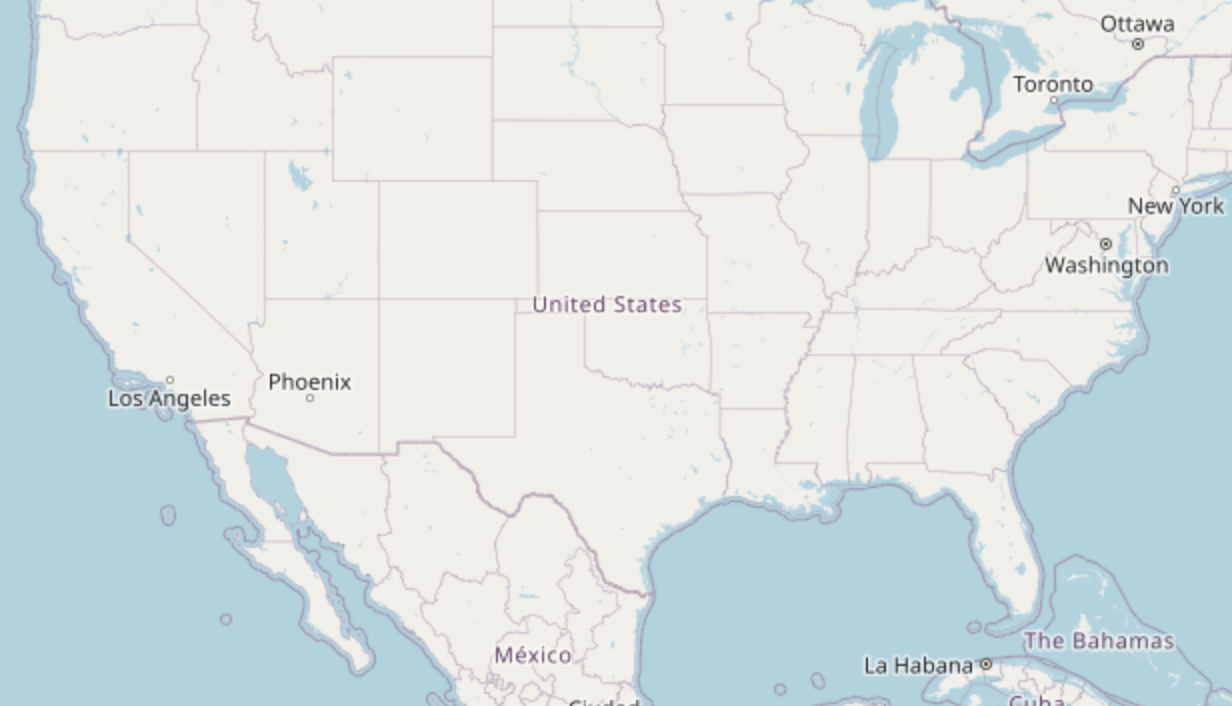
\includegraphics[width=0.9\linewidth]{img/osm1.png}
\end{figure}
City closest to the mean GPS coordinates -- does it protect privacy of the members?
\end{frame}


\begin{frame}{Example more concretely}
All cities $C$ = \{Ottawa (45, -75), Toronto, New York, Washington, Memphis (35, -90), Los Angeles, La Habana (23, -82)\}

\begin{table}
\footnotesize
\begin{tabular}{llc}
\toprule
Person & City & (Latitude, Longitude)\\ \midrule
Alice & Los Angeles & (34, -118) \\
Bob & New York & (40, -74) \\
Charlie & Washington & (38, -77) \\
Xander & Toronto & (43, -79) \\ \bottomrule
\end{tabular}
\caption{The Secret Society, database $D$}
\end{table}

Mean = 36, -88, closest city = Memphis (35, -90)

\end{frame}


\begin{frame}{Example more concretely}

\begin{figure}
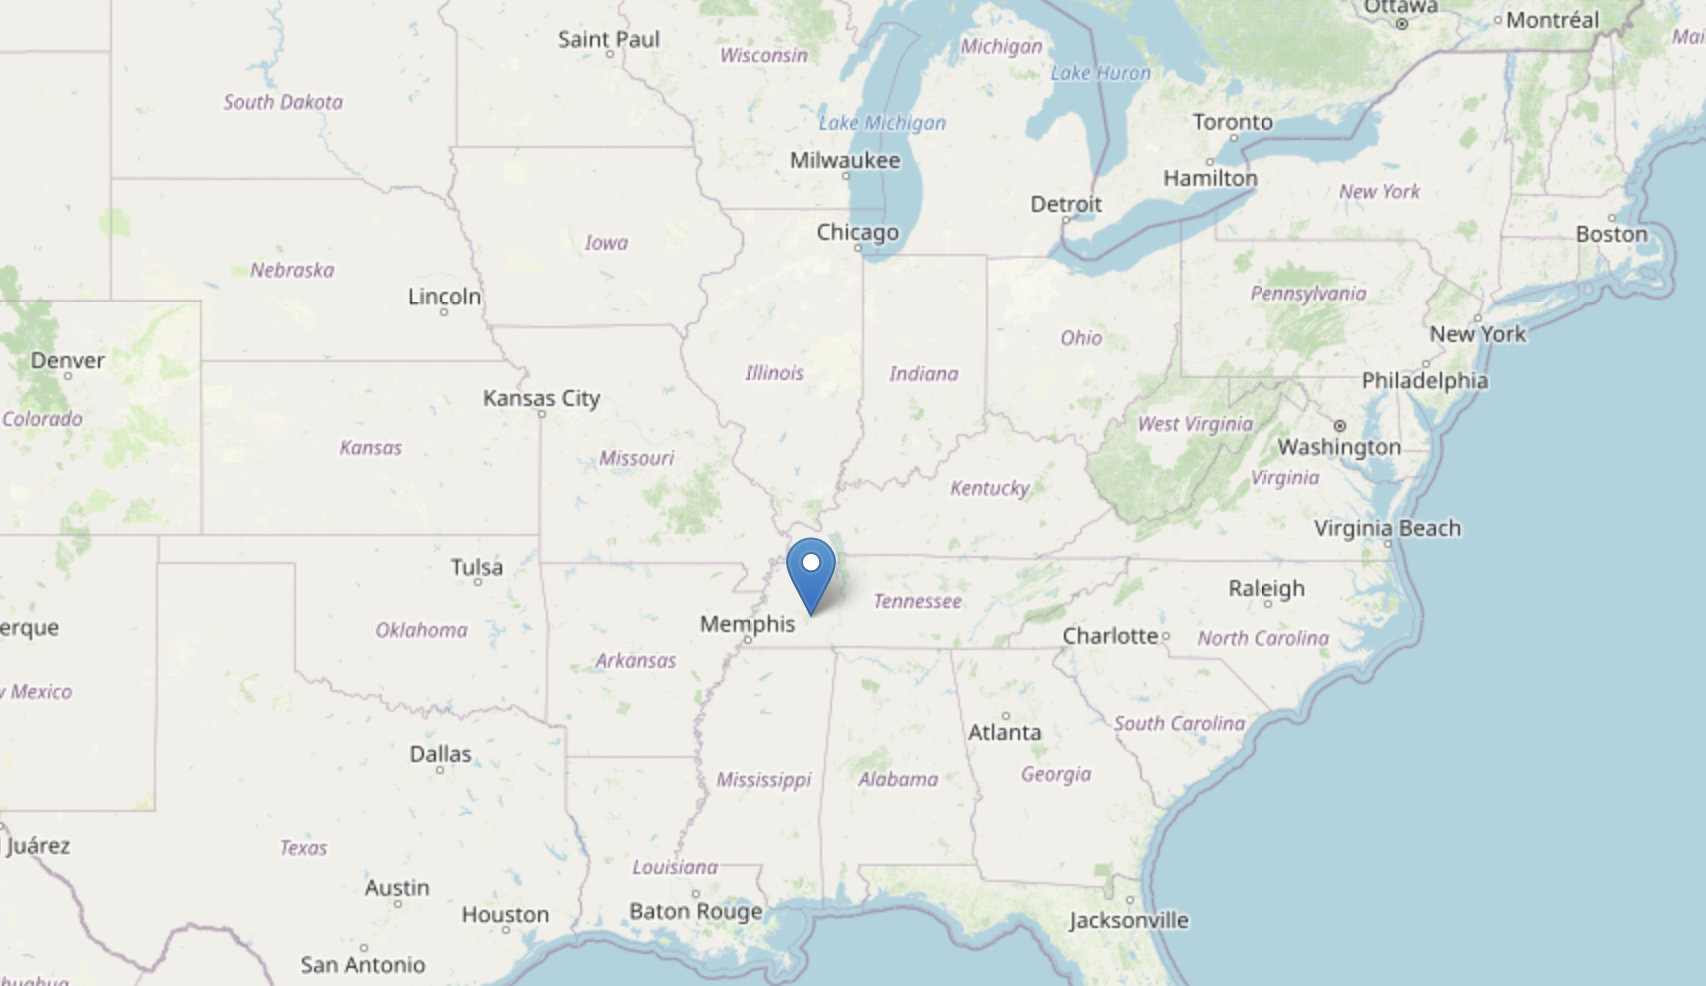
\includegraphics[width=0.9\linewidth]{img/osm2.png}
\end{figure}
Mean = 36, -88, closest city = Memphis (35, -90)

\end{frame}

\begin{frame}{Let's define a utility function}

Based on: Distance (Euclidian) of the database's $D$ GPS mean to a known city $c$ GPS
$$d(D, c)$$
(the smaller, the closer = better answer)

This is OK, but we want our utility $u$ to be higher for closer cities, so
$$
u(D, c) = \frac{1}{d(D, c)}
$$
(ignoring zero in the denominator for simplicity)

\end{frame}


\begin{frame}{Our query should return an element with highest utility}

Utility $u$: $u(D, c) = \frac{1}{d(D, c)}$

Take the database $D$, compute the mean coordinates, and choose city $c \in C$ with the highest utility.

What happens for a neighboring dataset $D'$?
\end{frame}


\begin{frame}{Does our utitily function have sensitivity?}
Utility formally: for a database and a range
$$
u: \mathcal{X} \times \mathcal{R} \to \mathbb{R}
$$

Sensitivity
$$
\Delta u = \max_{r \in \mathcal{R}} |u(D, r) - u(D', r)|
$$
for any neighboring datasets $D, D' \in \mathcal{X}$
\end{frame}

\begin{frame}{How to choose the city privately?}

\begin{block}{What we wanted}
Take the database $D$, compute the mean coordinates, and choose city $c \in C$ with the highest utility.
\end{block}

We want this process to be DP!

$\Pr[\mathcal{M}(D) =c] \leq \exp(\varepsilon) \Pr[\mathcal{M}(D') = c]$ for all neighboring datasets and any $c$

We need to sample $c$ somehow randomly
\end{frame}


\begin{frame}{Sample from a probability distribution over $\mathcal{R}$}

The Exponential mechanism
$$
\Pr [ \mathcal{M}(D) = r] = \frac{\exp \left( \frac{\varepsilon \cdot u(D, r)}{2 \Delta u} \right)}{\sum_{r' \in \mathcal{R}} \exp \left( \frac{\varepsilon \cdot u(D, r')}{2 \Delta u} \right)}
$$

Homework: Implement the example

Exercise: Proof that this is $(\varepsilon, 0)$-DP

\end{frame}






\begin{frame}{License and credits}

	\begin{columns}
		\begin{column}{0.7\textwidth}
			Licensed under Creative Commons Attribution-ShareAlike 4.0 International (CC BY-SA 4.0)
		\end{column}
		\begin{column}{0.2\textwidth}
			
\includegraphics[width=0.9\linewidth]{img/cc-by-sa-icon.pdf}
		\end{column}
	\end{columns}
	
	\bigskip
	
	Credits
	
	\begin{scriptsize}
		
		Ivan Habernal
		
		Content from ACL Anthology papers licensed under CC-BY \url{https://www.aclweb.org/anthology}
		
		Partly inspired by lectures from Antti Honkela, Aurélien Bellet, Gautam Kamath
	
	\end{scriptsize}
	
\end{frame}




\end{document}

